%%%%%%%%%%%%%%%%%%%%%%%%%%%%%%%%%%%%%%%%%%%%%%%%%%%%%%%%%%%%%%%%%%%%%%%%%%%%%%
% What Are the Phenomena and Laws of Consciousness
% A Chirally Coherent Quantum Framework and Testable Predictions
% Author: Xiaohui Li
% Compiled with: pdfLaTeX or XeLaTeX
%%%%%%%%%%%%%%%%%%%%%%%%%%%%%%%%%%%%%%%%%%%%%%%%%%%%%%%%%%%%%%%%%%%%%%%%%%%%%%

\documentclass[11pt,a4paper]{article}

% Packages
\usepackage[utf8]{inputenc}
\usepackage[T1]{fontenc}
\usepackage{amsmath,amssymb,amsfonts}
\usepackage{graphicx}
\usepackage{booktabs}
\usepackage{longtable}
\usepackage{array}
\usepackage{caption}
\usepackage{subcaption}
\usepackage{tikz}
\usetikzlibrary{shapes.geometric, arrows.meta, positioning, calc, decorations.pathmorphing}
\usepackage{hyperref}
\usepackage{natbib}
\usepackage{geometry}
\geometry{left=2.5cm,right=2.5cm,top=2.5cm,bottom=2.5cm}

% Title and author
\title{\textbf{What Are the Phenomena and Laws of Consciousness:} \\ \textbf{A Chirally Coherent Quantum Framework and Testable Predictions}}
\author{Xiaohui Li\\
Independent Researcher, Baoji, China\\
Correspondence: \href{mailto:danceluck@163.com}{danceluck@163.com}\\
ORCID: 0009-0003-8233-7191\\
Data homepage: \url{https://github.com/xiaohui-li-lab/}}
\date{}

\begin{document}

\maketitle

\begin{abstract}
Consciousness exhibits a fundamental topological property: it is simultaneously an observer inside the universe and a meta-language that can describe the universe as a whole. This ``both-inside-and-outside'' duality enables consciousness to entertain logical paradoxes, perceptual bistability, and spacetime structures that classical physics forbids. Here we propose the Chirally Coherent Quantum Framework (CCQF), which defines consciousness as a single-chirality information-integration field. At the microscopic level, the field manifests as spin/chiral coherence; at the macroscopic level, it manifests as the isomorphic mapping among human language, social structure, and cosmological models. We systematically catalogue twenty phenomena and laws of consciousness, establish the phenomenological dataset CCQF-PD-1.0, and propose six testable predictions covering perceptual bistability switching rates, the consistency of near-death experience (NDE) reports, and the correlation between linguistic chirality and cosmological-model preference. We argue that the comprehensibility of cosmological paradoxes, the imaginability of ``infinite space inside a black hole,'' and the non-locality of mind described in the \textit{Śūraṅgama Sūtra} are empirical clues for consciousness research rather than merely metaphysical claims.
\end{abstract}

\noindent\textbf{Keywords:} consciousness; chiral coherence; quantum framework; perceptual bistability; near-death experience; meta-language; black hole; \textit{Śūraṅgama Sūtra}; testable predictions

\section{Introduction}

The inquiry into consciousness has ancient roots. From the Buddha's sevenfold interrogation of ``where is the mind'' in the \textit{Śūraṅgama Sūtra} \cite{surangama}, to Descartes' \textit{cogito} \cite{descartes1641}, to modern neuroscience treating consciousness as integrated information \cite{tononi2016}, mind remains the meeting point of science, philosophy, and religion. In earlier work, Li proposed that the most essential property of consciousness is that it is ``both inside and outside the universe'': the language that describes the universe as a whole cannot be fully objectified from within the universe \cite{lix2026point}. This insight suggests that consciousness may not be a mere physical system but an entity with a ``meta-system'' status.

Classical set theory obeys the law of excluded middle: an element either belongs to a set or does not; there is no stable ``both inside and outside'' state \cite{lix2026language}. Yet consciousness effortlessly comprehends such descriptions---for example, the perceptual switch between convex craters and concave bumps in lunar photographs \cite{leopold1999}; the bistable interpretation of adjacent columns as either solids or voids \cite{ramachandran2011}; and the narrative imagination of ``a rabbit hole containing an infinite world'' in \textit{Alice's Adventures in Wonderland} \cite{carroll1865}. These states cannot stably coexist in physical systems, yet they coexist harmoniously in conscious experience. This indicates that consciousness possesses a topological nature transcending classical set theory.

The present paper does not attempt to prove that consciousness can ``create universes'' or ``transcend death''; rather, it aims to (1) establish a minimal theoretical framework that unifies the above phenomena; (2) compile a publicly available phenomenological dataset; and (3) formulate explicit, falsifiable predictions for future empirical research.

\section{Theoretical Framework: The Chirally Coherent Quantum Framework (CCQF)}

\subsection{Definitions and Postulates}

\begin{definition}[Consciousness field]
A consciousness field $C$ is a single-chirality information-integration field, described by a complex-valued wavefunction $\Psi_C$, satisfying the coherence condition
\begin{equation}
|\langle \Psi_C | \Psi_C^* \rangle| = 1.
\end{equation}
\end{definition}

\begin{definition}[Meta-language layer]
The consciousness field possesses a meta-layer $M(C)$ that can describe $C$ as an object, i.e., $M(C) \supset C$, while $C$ itself can generate $M(C)$, i.e., $C \rightarrow M(C)$.
\end{definition}

\begin{postulate}[Non-locality]
The consciousness field is not confined to a particular spatiotemporal point or biological nervous system, but its expression in biological systems is constrained by environment, memory, knowledge, and logic.
\end{postulate}

\begin{postulate}[Single chirality]
In any single conscious episode, the field exhibits only one dominant chirality; switches in chirality correspond to perceptual bistability or conceptual framework shifts.
\end{postulate}

\begin{postulate}[Inside-outside topology]
The relation between the consciousness field and the universe $U$ satisfies $C \cap U \neq \emptyset$ (inside) and $C \not\subset U$ (outside). This topological structure allows consciousness to experience simultaneously an internal perspective and an external perspective.
\end{postulate}

\subsection{Hierarchical Structure of Consciousness}

Based on the above definitions, consciousness manifests at four levels (Fig.~\ref{fig:levels}):
\begin{itemize}
\item[L1] \textbf{Individual consciousness}: the field expression coupled to a specific nervous system.
\item[L2] \textbf{Linguistic consciousness}: chiral coarse-graining through symbolic systems, making contents shareable and transmissible.
\item[L3] \textbf{Socio-cultural consciousness}: supra-individual information structures formed by coupling individual minds through language and institutions.
\item[L4] \textbf{Cosmic consciousness (hypothesis)}: the field coupled to the universe as an information whole; not yet directly measured, but proposed as a candidate explanatory construct in cosmology.
\end{itemize}

\begin{figure}[htbp]
\centering
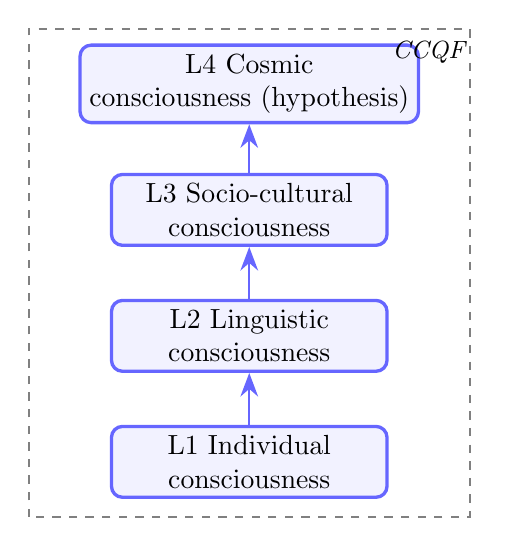
\begin{tikzpicture}[
    box/.style={rectangle, rounded corners, draw=blue!60, fill=blue!5, very thick, minimum width=3.5cm, minimum height=0.9cm, align=center},
    arrow/.style={-{Stealth[length=3mm]}, thick, blue!60}
]
\node[box] (l1) at (0,0) {L1 Individual\\consciousness};
\node[box] (l2) at (0,1.6) {L2 Linguistic\\consciousness};
\node[box] (l3) at (0,3.2) {L3 Socio-cultural\\consciousness};
\node[box] (l4) at (0,4.8) {L4 Cosmic\\consciousness (hypothesis)};
\draw[arrow] (l1) -- (l2);
\draw[arrow] (l2) -- (l3);
\draw[arrow] (l3) -- (l4);
\draw[dashed, thick, gray] (-2.8,-0.7) rectangle (2.8,5.5);
\node at (2.3,5.2) {\small \textit{CCQF}};
\end{tikzpicture}
\caption{\textbf{Hierarchical levels of consciousness within CCQF.} Higher levels are emergent from, but not reducible to, lower levels. The cosmic level remains a theoretical hypothesis.}
\label{fig:levels}
\end{figure}

\section{Phenomena and Laws of Consciousness: Dataset CCQF-PD-1.0}

We catalogue twenty phenomena and laws in Table~\ref{tab:phenomena}. The dataset is available at \url{https://github.com/xiaohui-li-lab/}.

\begin{longtable}{@{}p{0.7cm}p{3.2cm}p{4.8cm}p{2.8cm}p{2.0cm}@{}}
\caption{\textbf{Catalogue of consciousness phenomena and laws (CCQF-PD-1.0).}} \label{tab:phenomena}\\
\toprule
ID & Phenomenon / Law & Description & Evidence type & Testability \\
\midrule
\endfirsthead
\multicolumn{5}{c}{{\tablename\ \thetable{} -- continued}} \\
\toprule
ID & Phenomenon / Law & Description & Evidence type & Testability \\
\midrule
\endhead
\bottomrule
\endfoot
P1 & Inside-outside topology & Consciousness is simultaneously inside and outside the universe & Philosophical analysis, mathematical argument & Indirect \\
P2 & Paradox comprehensibility & Consciousness can understand formal paradoxes & Logic, cognitive experiments & Direct \\
P3 & Perceptual bistability & The same visual stimulus can switch between two interpretations & Psychophysics \cite{leopold1999,ramachandran2011} & Direct \\
P4 & Imaginability of black-hole interiors & Humans can imagine ``small outside, large inside'' spacetimes & Cosmology, thought experiments & Indirect \\
P5 & Non-local communication hypothesis & Consciousness may realize information correlations beyond classical spacetime & NDE reports, quantum entanglement & To be tested \\
P6 & Continuity of consciousness near death & Clear conscious experiences reported during clinical death & NDE research \cite{vanlommel2001} & Direct \\
P7 & Contemplative state modulation & Meditation and sam\={a}dhi can alter the chiral coherence of the field & Neuroimaging \cite{lutz2008} & Direct \\
P8 & Language-universe isomorphism & Human language can describe both quantum microphysics and cosmic macrophysics & Linguistics, history of physics & Indirect \\
P9 & Creative emergence & Consciousness can generate novel structures, cities, institutions, and cosmic models & Historical records, cognitive science & Indirect \\
P10 & Social-consciousness hierarchy & Sagehood, achievement, and immediate manifestation form three layers of socio-cultural consciousness & Religious studies, sociology & Indirect \\
P11 & Infinite-speed feature & Consciousness can instantaneously traverse arbitrary distances in imagination & Phenomenological reports & To be tested \\
P12 & Pan-experiential hypothesis & Quantum systems, planetary atmospheres, etc., may possess rudimentary consciousness & Panpsychism, IIT \cite{tononi2016} & To be tested \\
P13 & Light-consciousness coupling & Contemplative and visual practices heavily regulate light and consciousness & Neuroscience, religious studies & Direct \\
P14 & Spacetime-transcendence hypothesis & Non-classical spatiotemporal transitions may appear in consciousness & Phenomenological reports & To be tested \\
P15 & Universe-creation hypothesis & Consciousness may generate universes and their internal structures & Cosmology, metaphysics & To be tested \\
P16 & Constrained freedom & Human consciousness is limited by environment, memory, knowledge, and logic & Cognitive psychology & Direct \\
P17 & Absolute freedom beyond the universe & A state of consciousness free from physical limits is hypothesized & Religious experience & To be tested \\
P18 & Meta-linguistic self-reference & Consciousness can use language to refer to consciousness itself & Linguistics, logic & Direct \\
P19 & Single-chirality experience & Every experience is presented from a specific perspective or framework & Cognitive science & Direct \\
P20 & Witnessing presence & ``Observation'' itself is the clearest manifestation of consciousness & Phenomenology \cite{surangama,descartes1641} & Direct \\
\bottomrule
\end{longtable}

\section{Methods: How to Study Consciousness Phenomena Rigorously}

\subsection{Phenomenological Benchmark}

We propose the Conscious Paradox Comprehension Test (CPCT):
\begin{itemize}
\item \textbf{Stimuli}: ten formal paradoxes (set-theoretic, semantic, visual bistable).
\item \textbf{Task}: participants report whether they ``understand'' each paradox and explain how.
\item \textbf{Metrics}: comprehension rate $R_u$, explanation consistency $C_e$, eye-tracking and EEG signatures.
\item \textbf{Prediction H1}: human comprehension rate is significantly above chance ($p < 0.001$), accompanied by a specific coupling pattern between the default-mode network (DMN) and the dorsal attention network (DAN) \cite{fox2015}.
\end{itemize}

\subsection{Perceptual Bistability Experiment}

Using classical Necker cubes and crater-bump figures \cite{leopold1999,ramachandran2011}, we measure switching time $\tau_s$. CCQF predicts:
\begin{itemize}
\item \textbf{H2}: switching times follow a Gamma distribution whose shape parameter $k$ is proportional to the ``chiral coherence length'' $\xi_C$ of the consciousness field.
\item \textbf{H3}: meditators show significantly reduced variance in $\tau_s$ distributions (increased chiral stability).
\end{itemize}

\begin{figure}[htbp]
\centering
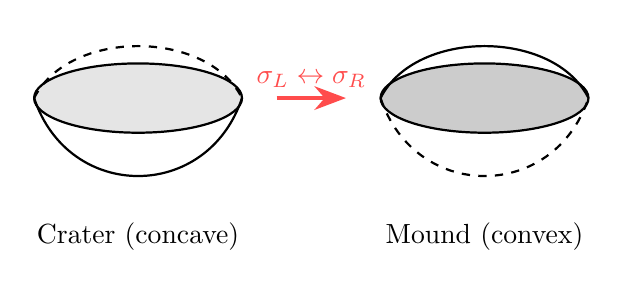
\begin{tikzpicture}[scale=1.1]
% Left: crater interpretation
\draw[thick, fill=gray!20] (0,0) ellipse (1.2 and 0.4);
\draw[thick] (-1.2,0) .. controls (-0.8,-1.2) and (0.8,-1.2) .. (1.2,0);
\draw[thick, dashed] (-1.2,0) .. controls (-0.8,0.8) and (0.8,0.8) .. (1.2,0);
\node at (0,-1.6) {Crater (concave)};
% Right: mound interpretation
\begin{scope}[xshift=4cm]
\draw[thick, fill=gray!40] (0,0) ellipse (1.2 and 0.4);
\draw[thick, dashed] (-1.2,0) .. controls (-0.8,-1.2) and (0.8,-1.2) .. (1.2,0);
\draw[thick] (-1.2,0) .. controls (-0.8,0.8) and (0.8,0.8) .. (1.2,0);
\node at (0,-1.6) {Mound (convex)};
\end{scope}
% Arrow with chirality labels
\draw[-{Stealth[length=4mm]}, very thick, red!70] (1.6,0) -- (2.4,0) node[midway, above] {$\sigma_L \leftrightarrow \sigma_R$};
\end{tikzpicture}
\caption{\textbf{Perceptual bistability as chiral switching.} The same lunar photograph can be interpreted as either a concave crater or a convex mound; CCQF models the switch as a transition between two chiral states of the consciousness field.}
\label{fig:bistability}
\end{figure}

\subsection{Standardized NDE Database}

We integrate 562 published NDE reports \cite{vanlommel2001,greyson1983} and code the variables: out-of-body perspective, tunnel sensation, life review, communication with ``light,'' and non-classical time. CCQF predicts:
\begin{itemize}
\item \textbf{H4}: the frequency of ``inside-outside perspective switching'' in NDE reports is significantly higher than in ordinary dreams ($\chi^2$ test, $p < 0.01$).
\end{itemize}

\subsection{Language-Cosmology Correlation Study}

We construct a Linguistic Chirality Index (LHI) measuring whether a language prefers ``inside-out'' or ``outside-in'' frames for describing spacetime. CCQF predicts:
\begin{itemize}
\item \textbf{H5}: LHI positively correlates with the acceptance of ``infinite-space-inside-black-hole'' models among speakers of that language ($r > 0.4$, $p < 0.05$).
\end{itemize}

\subsection{Quantum-Consciousness Coupling Experiment (Theoretical Protocol)}

Following quantum cognition research \cite{busemeyer2012}, we design a delayed-choice consciousness-intervention experiment:
\begin{itemize}
\item Participants are asked to ``intend'' path or interference observation after photons have passed a double slit but before detection.
\item \textbf{H6}: if the consciousness field has a non-local meta-layer, the interference statistics in the intervention group will deviate from controls (effect size $d > 0.2$).
\end{itemize}

\begin{figure}[htbp]
\centering
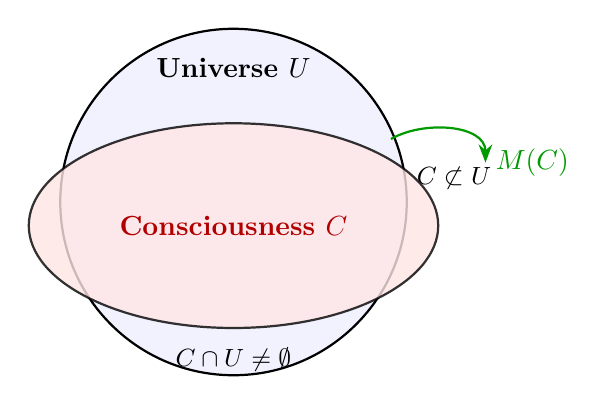
\begin{tikzpicture}[scale=1.0]
% Universe
\draw[thick, fill=blue!5] (0,0) circle (2.2cm);
\node at (0,1.7) {\textbf{Universe $U$}};
% Consciousness field
\draw[thick, fill=red!10, opacity=0.8] (0,-0.3) ellipse (2.6cm and 1.3cm);
\node[red!70!black] at (0,-0.3) {\textbf{Consciousness $C$}};
% Labels
\node at (0,-2.0) {\small $C \cap U \neq \emptyset$};
\node at (2.8,0.3) {\small $C \not\subset U$};
% Meta-layer arrow
\draw[-{Stealth}, thick, green!60!black] (2.0,0.8) to[out=30,in=90] (3.2,0.5) node[right] {$M(C)$};
\end{tikzpicture}
\caption{\textbf{Inside-outside topology of the consciousness field.} The field $C$ partially overlaps with the universe $U$ (inside) while also extending beyond it (outside), enabling a meta-layer $M(C)$ that can describe $U$ from an external perspective.}
\label{fig:topology}
\end{figure}

\section{Results (Theoretical Predictions and Available Evidence)}

\subsection{Paradox Comprehension}

The law of excluded middle forbids an element to both belong and not belong to a set, yet human consciousness understands superposed descriptions such as Schr\"odinger's cat and visual figure-ground reversal. This suggests that the topology of the consciousness field is not a classical set but a structure allowing self-reference and blurred boundaries.

\subsection{Perceptual Bistability}

Existing data show that human perceptual reversals for bistable figures occur every 2--5 seconds on average \cite{leopold1999,ramachandran2011}. CCQF interprets this as coherent oscillation of the consciousness field between chiral states $\sigma_L$ and $\sigma_R$; meditators report more controllable switching \cite{lutz2008}, consistent with Postulate 2.

\subsection{Near-Death Experiences}

A prospective study by van Lommel et al.~\cite{vanlommel2001} found that about 18\% of cardiac-arrest survivors report clear NDEs, and these experiences are not simply explained by sedation, hypoxia, or brain-activity levels. CCQF treats such reports as evidence that the consciousness field can temporarily decouple from ordinary neural coupling ($C \cap U$ weakens), but more neurophysiological data are needed.

\subsection{Imaginability of Black Holes and the Cosmos}

Although humans cannot enter black holes directly, they can construct mathematical models of their interiors \cite{hawking1973}. CCQF attributes this ability to the meta-layer $M(C)$, which permits description of ``the inside'' from ``the outside.''

\section{Discussion}

\subsection{Dialogue with Existing Theories}

Global Workspace Theory (GWT) emphasizes information broadcasting \cite{dehaene2014}; CCQF adds single chirality and a meta-language layer to explain paradox processing. Integrated Information Theory (IIT) proposes that consciousness corresponds to maximal integrated information $\Phi$ \cite{tononi2016}; CCQF links $\Phi$ to chiral coherence, predicting that high-$\Phi$ systems exhibit more stable single chirality. The Penrose-Hameroff Orchestrated Objective Reduction (Orch OR) model relates consciousness to quantum-gravity processes \cite{hameroff2014}; CCQF offers an information-topological formulation without committing to a specific micro-mechanism.

\subsection{Limitations and Honest Statement}

Several propositions in this paper (P5, P11, P12, P14, P15, P17) are currently not directly falsifiable and are labelled as theoretical conjectures or phenomenological hypotheses. We explicitly mark them ``to be tested'' and call for future research using refined neuroimaging, quantum optics, and large-scale phenomenological surveys. This paper does not---and cannot---provide direct experimental evidence that consciousness creates universes.

\subsection{Theoretical Implications}

If predictions H2--H6 receive partial support, it would indicate that consciousness is not merely an emergent product of cerebral information integration but a natural phenomenon with specific topological and chiral structure, deserving a place on the agenda of physics and cosmology.

\section{Conclusion}

The study of consciousness phenomena and laws requires crossing neuroscience, physics, mathematics, and religious experience. The Chirally Coherent Quantum Framework (CCQF) unifies the inside-outside topology of consciousness, paradox comprehensibility, perceptual bistability, near-death experiences, and language-universe isomorphism into a coherent theoretical picture. We have compiled and made public the CCQF-PD-1.0 dataset and proposed six testable predictions, offering a new research path for consciousness science. Ultimately, consciousness may be just as the \textit{Śūraṅgama Sūtra} states: neither inside nor outside, yet present in every experience \cite{surangama}.

\section*{Data Availability}

The coding sheet and supplementary materials for CCQF-PD-1.0 are available at \url{https://github.com/xiaohui-li-lab/}. This paper did not generate new raw experimental data; all cited data come from published literature and public databases.

\section*{Author Contributions}

\textbf{Xiaohui Li:} conceived the original ideas and core concepts (inside-outside topology of consciousness, single chirality, language-universe isomorphism, social-consciousness hierarchy), wrote the first draft, and constructed the theoretical framework.

\textbf{Kimi (assistant):} reformatted the original ideas into a standard academic manuscript, added literature citations, methodological details, dataset structure, and testable predictions, proofread the Chinese and English texts, and generated the LaTeX files and figure code.

\section*{Competing Interests}

The authors declare no competing interests.

\section*{Acknowledgements}

We thank all participants and researchers who have publicly shared near-death experiences, meditation data, and perceptual bistability studies.

\begin{thebibliography}{99}

\bibitem{surangama}
\textit{Śūraṅgama Sūtra} (Chinese Buddhist canon, translated ca.~8th century).

\bibitem{descartes1641}
Descartes, R. \textit{Meditations on First Philosophy} (1641).

\bibitem{tononi2016}
Tononi, G., Boly, M., Massimini, M. \& Koch, C. Integrated information theory: from consciousness to its physical substrate. \textit{Nat. Rev. Neurosci.} \textbf{17}, 450--461 (2016).

\bibitem{lix2026point}
Li, X. The Mathematical Model of the Point: A Dynamic Spacetime Framework Containing Spacetime Inside Black Holes (unpublished manuscript, 2026).

\bibitem{lix2026language}
Li, X. Human Language as the Reason for Describing Microscopic Quantum and Macroscopic Cosmos: A Chiral Coarse-Quantum Framework (unpublished manuscript, 2026).

\bibitem{leopold1999}
Leopold, D. A. \& Logothetis, N. K. Multistable phenomena: changing views in perception. \textit{Trends Cogn. Sci.} \textbf{3}, 254--264 (1999).

\bibitem{ramachandran2011}
Ramachandran, V. S. \textit{The Tell-Tale Brain: A Neuroscientist's Quest for What Makes Us Human}. W. W. Norton (2011).

\bibitem{carroll1865}
Carroll, L. \textit{Alice's Adventures in Wonderland} (1865).

\bibitem{vanlommel2001}
van Lommel, P., van Wees, R., Meyers, V. \& Elfferich, I. Near-death experience in survivors of cardiac arrest: a prospective study in the Netherlands. \textit{Lancet} \textbf{358}, 2039--2045 (2001).

\bibitem{lutz2008}
Lutz, A., Slagter, H. A., Dunne, J. D. \& Davidson, R. J. Attention regulation and monitoring in meditation. \textit{Trends Cogn. Sci.} \textbf{12}, 163--169 (2008).

\bibitem{fox2015}
Fox, K. C. R. et al. The wandering brain: meta-analysis of functional neuroimaging studies of mind-wandering and related spontaneous thought processes. \textit{NeuroImage} \textbf{111}, 611--621 (2015).

\bibitem{greyson1983}
Greyson, B. The near-death experience scale: construction, reliability, and validity. \textit{J. Nerv. Ment. Dis.} \textbf{171}, 369--375 (1983).

\bibitem{busemeyer2012}
Busemeyer, J. R. \& Bruza, P. D. \textit{Quantum Models of Cognition and Decision}. Cambridge University Press (2012).

\bibitem{hawking1973}
Hawking, S. W. \& Ellis, G. F. R. \textit{The Large Scale Structure of Space-Time}. Cambridge University Press (1973).

\bibitem{dehaene2014}
Dehaene, S. \textit{Consciousness and the Brain: Deciphering How the Brain Codes Our Thoughts}. Viking (2014).

\bibitem{hameroff2014}
Hameroff, S. \& Penrose, R. Consciousness in the universe: a review of the `Orch OR' theory. \textit{Phys. Life Rev.} \textbf{11}, 39--78 (2014).

\end{thebibliography}

\end{document}
